% !Rnw weave = knitr
% !TEX TS-program = lualatex
% !TEX encoding = UTF-8 Unicode

\documentclass{article}\usepackage[]{graphicx}\usepackage[]{color}
% maxwidth is the original width if it is less than linewidth
% otherwise use linewidth (to make sure the graphics do not exceed the margin)
\makeatletter
\def\maxwidth{ %
  \ifdim\Gin@nat@width>\linewidth
    \linewidth
  \else
    \Gin@nat@width
  \fi
}
\makeatother

\definecolor{fgcolor}{rgb}{0.345, 0.345, 0.345}
\newcommand{\hlnum}[1]{\textcolor[rgb]{0.686,0.059,0.569}{#1}}%
\newcommand{\hlstr}[1]{\textcolor[rgb]{0.192,0.494,0.8}{#1}}%
\newcommand{\hlcom}[1]{\textcolor[rgb]{0.678,0.584,0.686}{\textit{#1}}}%
\newcommand{\hlopt}[1]{\textcolor[rgb]{0,0,0}{#1}}%
\newcommand{\hlstd}[1]{\textcolor[rgb]{0.345,0.345,0.345}{#1}}%
\newcommand{\hlkwa}[1]{\textcolor[rgb]{0.161,0.373,0.58}{\textbf{#1}}}%
\newcommand{\hlkwb}[1]{\textcolor[rgb]{0.69,0.353,0.396}{#1}}%
\newcommand{\hlkwc}[1]{\textcolor[rgb]{0.333,0.667,0.333}{#1}}%
\newcommand{\hlkwd}[1]{\textcolor[rgb]{0.737,0.353,0.396}{\textbf{#1}}}%
\let\hlipl\hlkwb

\usepackage{framed}
\makeatletter
\newenvironment{kframe}{%
 \def\at@end@of@kframe{}%
 \ifinner\ifhmode%
  \def\at@end@of@kframe{\end{minipage}}%
  \begin{minipage}{\columnwidth}%
 \fi\fi%
 \def\FrameCommand##1{\hskip\@totalleftmargin \hskip-\fboxsep
 \colorbox{shadecolor}{##1}\hskip-\fboxsep
     % There is no \\@totalrightmargin, so:
     \hskip-\linewidth \hskip-\@totalleftmargin \hskip\columnwidth}%
 \MakeFramed {\advance\hsize-\width
   \@totalleftmargin\z@ \linewidth\hsize
   \@setminipage}}%
 {\par\unskip\endMakeFramed%
 \at@end@of@kframe}
\makeatother

\definecolor{shadecolor}{rgb}{.97, .97, .97}
\definecolor{messagecolor}{rgb}{0, 0, 0}
\definecolor{warningcolor}{rgb}{1, 0, 1}
\definecolor{errorcolor}{rgb}{1, 0, 0}
\newenvironment{knitrout}{}{} % an empty environment to be redefined in TeX

\usepackage{alltt}
\usepackage[utf8]{inputenc}
\usepackage[english]{babel}
\usepackage{fontspec}
\usepackage{geometry, graphicx}
 % you must load Sweave with the `noae` option

\usepackage{hyperref}
\hypersetup{
    colorlinks=true,
    linkcolor=blue,
    filecolor=magenta,      
    urlcolor=cyan,
}

\title{Lab 1: Intro to R}
\author{David Sichinava}
\date{\today}
\IfFileExists{upquote.sty}{\usepackage{upquote}}{}
\begin{document}



% \SweaveOpts{concordance=TRUE}
\maketitle
\section*{Topics}
\begin{itemize}
\item Intro to R
\item R GUI: R-Studio
\item Creating R markdown documents
\item Literate programming
\end{itemize}

\section*{Instruction:}

\paragraph{}
Follow the assignment step-by-step. Name your $.rmd$ file in a following format: $your\_surname\_lab1.rmd$. For example,

\begin{knitrout}
\definecolor{shadecolor}{rgb}{0.969, 0.969, 0.969}\color{fgcolor}\begin{kframe}
\begin{alltt}
\hlstd{sichinava_lab1.Rmd}
\end{alltt}
\end{kframe}
\end{knitrout}

\section*{Assignments:}

\subsection*{File system and navigation:}
\paragraph{}
First of all, create a working directory for your work in your computer. As we are going to have assignment for each lab, create a separate folder for this class $intro\_stats\_r4$, add a subfolder $labs$ and create a folder for the first lab: $lab\_1$.
\begin{figure}[h]
\centering
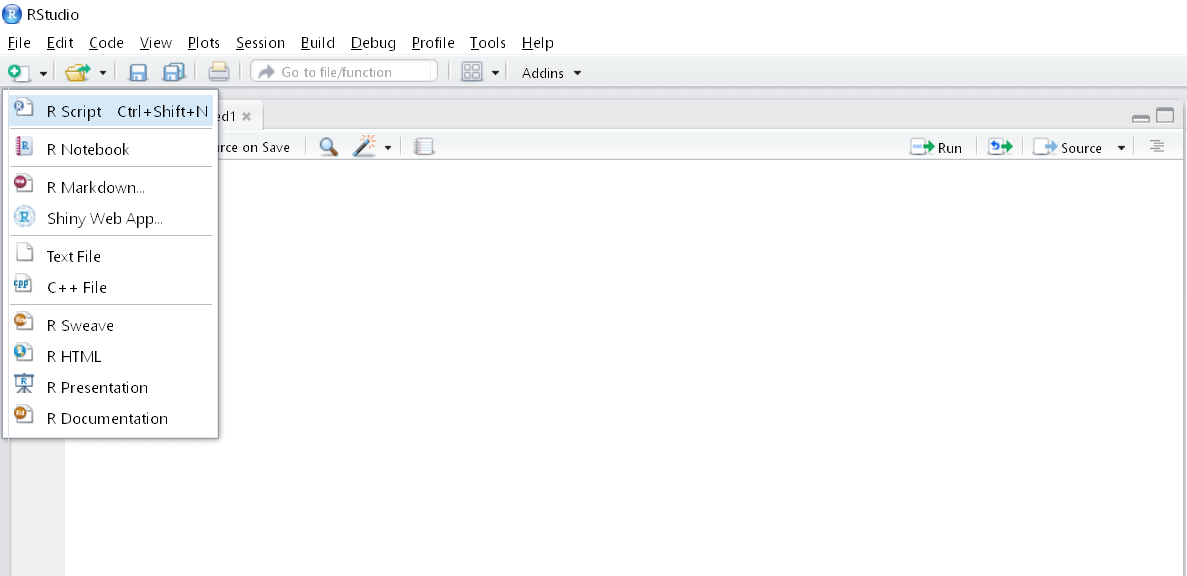
\includegraphics[width=\textwidth]{img/new_menu.PNG}
\caption{Creating a new file}
    \label{create:file}
\end{figure}
\paragraph{}
Open `R-studio` and create new $R$-notebook. Assign a name and save it into $lab\_1$ folder. Saving is simple: you just click a corresponding icon in a menu and select necessary format (See picture. \ref{create:file}).
Cool! Now in the notebook, after the preamble (see picture \ref{preamble}) type a short text about your impressions on $R-Studio$. Two or three sentences are enough.
\begin{figure}[h]
\centering
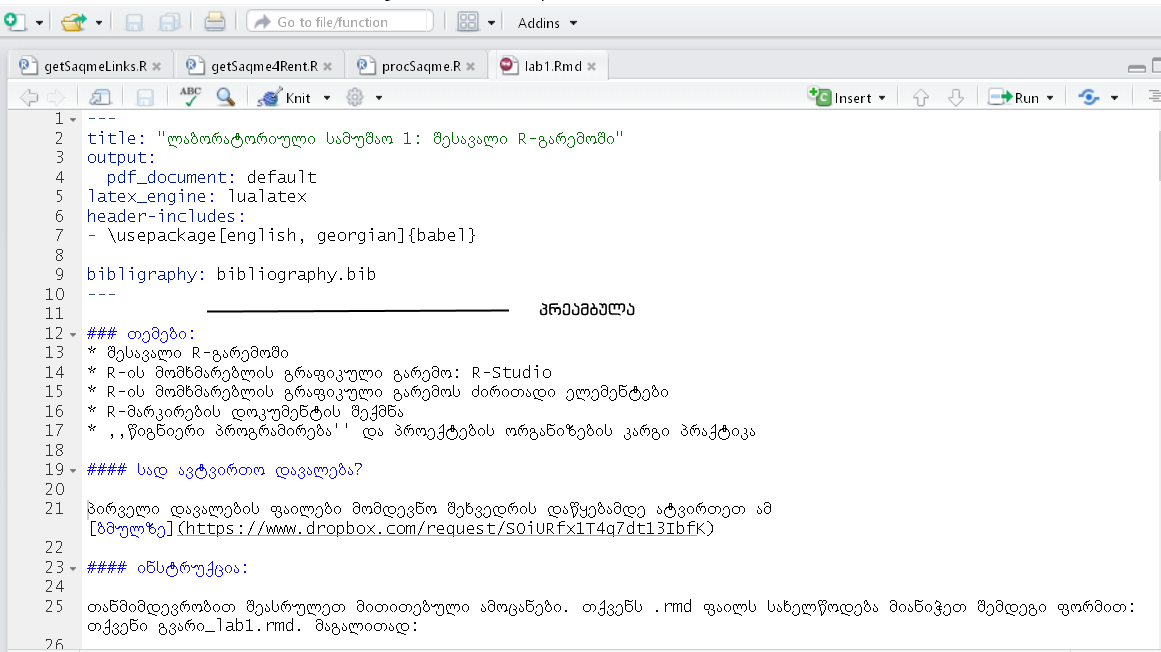
\includegraphics[width=\textwidth]{img/preamble.PNG}
\caption{Document preamble}
    \label{preamble}
\end{figure}
\paragraph{}
Insert code chunk in your notebook. Be sure that your code is active. In order to check that look on a green button on the right side of the chunk (see picture \ref{chunk}). Write down a code between accent marks which will navigate you to your working directory.


\subsection*{Installing and activating libraries}
\paragraph{}
Insert new code chunk in your notebook. Write down a code which will install $ggplot2$ library. Run the code and make sure it works.

In a new line write a code which will activate $ggplot2$. Run the code and again make sure it runs for you.


\subsection*{Creating a script file and sourcing}

Click a button for creating new file and select $R$ script file. R script is just a text file where we type our code, which can be opened in R environment and executed (sourced) In difference with markdown document, we cannot have a $rich text$ in script files. Usually we don't include text in the script, file, however you can have one by $commenting$ it. (see figure \ref{comment}). The program will ignore script lines with leading hashtags.

\begin{figure}[h]
\centering
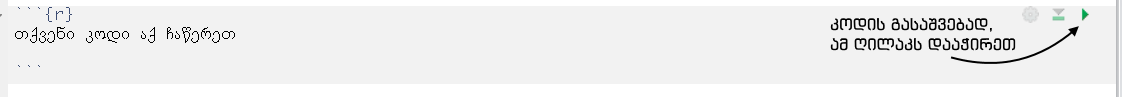
\includegraphics[width=\textwidth]{img/run_chunk.PNG}
\caption{Selecting and running code chunk}
    \label{chunk}
\end{figure}

In the script file, write a code which will install $tidyr$ library and activate it. Create a new subfolder $source$ in your $lab\_1$ folder and save your script file there. Give a reasonable name and extension $.R$ to the script file.

According to the principles of literate programming, we should run (or, in R-speak, $source$) the script from notebook. In order to do that, go back to the notebook, add a code chunk, type the code which will run the script, and make sure that it runs correctly.

\subsection*{Processing the document}

In order to follow the principles of literatre programming, in the notebook write a short description right before each code chunk. Just describe in plain words what each of the chunks are supposed to do. Do not limit yourself to plain text. Use wide formatting possibilities of markdown, for example, mark sections, insert links, pictures, bold and italic texts. Each of this will earn you extra points.

In order to acquaint yourself to the possibilities of Markdown, navigate to \href{https://www.rstudio.com/wp-content/uploads/2016/03/rmarkdown-cheatsheet-2.0.pdf}{this link} or  \href{https://github.com/adam-p/markdown-here/wiki/Markdown-Cheatsheet}{check out this link}.

\begin{figure}[h]
\centering
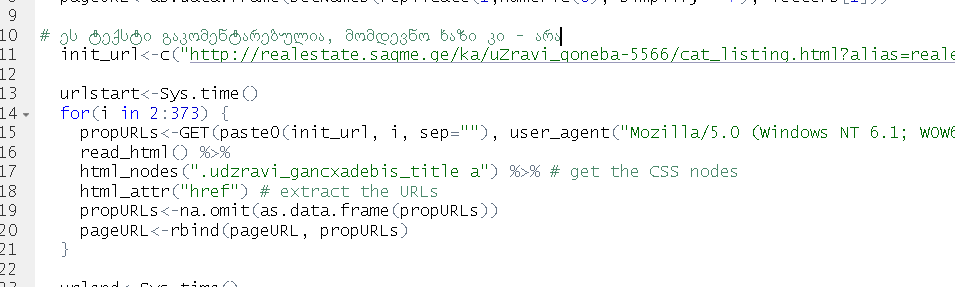
\includegraphics[width=\textwidth]{img/commented.PNG}
\caption{Commenting the code}
    \label{comment}
\end{figure}



\subsection*{Compiling the document}

Before you compile the document, that is, transfer it into $.html$ format, save your notebook (just click $save$ button or hit $ctrl+S$). $.html$ or HyperText Markup Language is a standard language for creating websites. That said, your compiled document could be opened in any relatively modern web browser.

\begin{figure}[h]
\centering
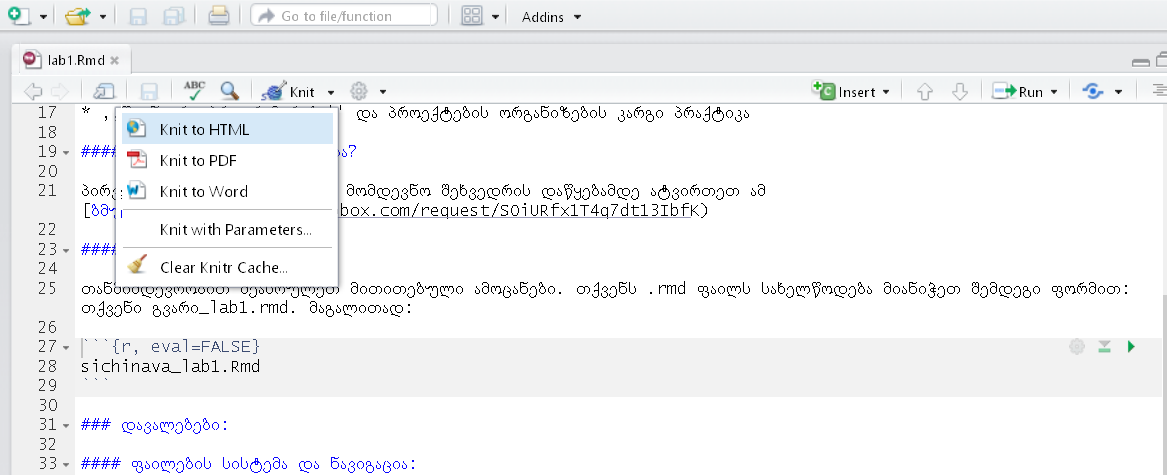
\includegraphics[width=\textwidth]{img/knit_to_html.PNG}
\caption{Compiling the document}
    \label{compile}
\end{figure}

In order to compile the document, hit the knit button and select \emph{knit to HTML} (see figure \ref{compile}. If you did everything correctly, your compiled notebook will load automatically. Remember that when compiling, R-Studio executes all the code written in the document.

\subsection*{Annotated bibliography}

You can type the text for the annotated bibliography directly into R-notebook. Use APA standards and the following example to prepare the bibliography:

Brenner, N., & Theodore, N. (2002). Cities and the geographies of “actually existing neoliberalism”. _Antipode, 34(3), 349-379._


The authors, researchers at the Rand Corporation and Brown University, use data from the National Longitudinal Surveys of Young Women and Young Men to test their hypothesis that nonfamily living by young adults alters their attitudes, values, plans, and expectations, moving them away from their belief in traditional sex roles. They find their hypothesis strongly supported in young females, while the effects were fewer in studies of young males. Increasing the time away from parents before marrying increased individualism, self-sufficiency, and changes in attitudes about families. In contrast, an earlier study by Williams cited below shows no significant gender differences in sex role attitudes as a result of nonfamily living.

\emph{Example source: http://guides.library.cornell.edu/annotatedbibliography)}

Here are the three articles which you have to read and write bibliography:

\begin{itemize}
\item Goodman, S. N., Fanelli, D., & Ioannidis, J. P. (2016). \href{https://www.dropbox.com/s/4io57pvabqw539s/Goodman%2C%202016.pdf?dl=0)}{What does research reproducibility mean?}. \emph{Science translational medicine}, 8(341).
\item  Iqbal, S. A., Wallach, J. D., Khoury, M. J., Schully, S. D., & Ioannidis, J. P. (2016). \href{https://www.dropbox.com/s/dgl3tbskfjjn5ib/iqbal_et_al%2C%202016.PDF?dl=0}{Reproducible research practices and transparency across the biomedical literature}. \emph{PLoS Biol}, 14(1).
\item  Stodden, V. (2010). \href{https://www.dropbox.com/s/uh7vd6diud8tcyu/Stodden%2C%202010.pdf?dl=0}{Data sharing in social science repositories: facilitating reproducible computational research}. \emph{NIPS} 2010.
\end{itemize}

After you are done with writing the text. Compile the document. Remember that previous $.html$ file will be overwritten.

\subsection*{Done. How to submit my assignment?}

Zip the whole folder for the first lab. Name the file according to the following format: $surname\_lab1.zip$ like this:

\begin{knitrout}
\definecolor{shadecolor}{rgb}{0.969, 0.969, 0.969}\color{fgcolor}\begin{kframe}
\begin{alltt}
\hlstd{sichinava_lab1.zip}
\end{alltt}
\end{kframe}
\end{knitrout}

Upload the file to \href{https://www.dropbox.com/request/fJXwi6SVJ0D7r1WvxyG9}{this link} before the start of our next meeting.


Good luck!


\end{document}
